
\subsection{Equivalence of NFAs and DFAs}
% ------------------------------------------------------------

A finite automaton(DFA $\Longleftrightarrow$ NFA)

\begin{enumerate}
    \item Defining Models of computation.
    \item testifying equivalence between models.
\end{enumerate}

\begin{definition}[Reverse] \ \\
    \begin{compactitem}
    \item
        reverse of a string
            \[
                \rev\big( \lst{Q_1, Q_2, \cdots, Q_n} \big) = \lst{Q_n,  Q_(n-1), \cdots,
                Q_1}.
            \]
    \item
        reverse of a language
            \[
                \rev(L) = \set{ rev(w) \mid w \in L }.
            \]
         \myfigure{Example of NFA}{pics/mp/nfa-2.pdf}
    \end{compactitem}
\end{definition}

It is easy to find out that 
\[
    \forall L \in \mathbb R, \rev(L) \in \mathbb R.
        \footnote{$\mathbb R $ = Regular language}
\]

\begin{example}[Regular language is closed under union]
    \label{exa:R_closed_under_union_with_NFA}

    Recall \autoref{exa:R_closed_under_union}, with NFA, we could proof
    \autoref{thm:R_closed_under_union} much more easier now.

    \begin{proof}[Proof of \autoref{thm:R_closed_under_union}]
        Let $M_1, M_2$ become NFA for $L_1$ and $L_2$.
        We build a NFA for $L_1 \cup L_2$
        by simply adding a new initial state that transit to $s_1$ and $s_2$ with
        $\varepsilon$ arrows:
        \centgraph[3cm]{pics/mp/nfa-3.pdf}
    \end{proof}
\end{example}



\begin{example}[Regular language is closed under concatenation]
    \begin{proof}
        Let $M_1, M_2$ become NFA for $L_1$ and $L_2$.
        We build a NFA for $L_1 \circ L_2$:
        \begin{compactenum}
        \item Assign M's start to be the start state of $M_1$ which is $s_1$ and
        \item change the final states in $M_1$ to regular states and connect them to $s_2$
            with additional $\varepsilon$ arrows that nondeterministically allow branching
            to $M_2$ whenevr $M_1$ is in an accept state, signifying that it has found an
            initial piece of the input that constitues a string in $L_1$
        \item The accept states of $M$ are the accept states of $M_2$ only. only.
        \end{compactenum}
        See the graph for visualization:
        \begin{center}
            \begin{minipage}{4cm}
                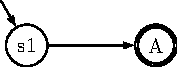
\includegraphics[width=\textwidth]{pics/mp/nfa-4.pdf}
                \center $M_1$
                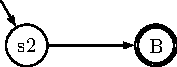
\includegraphics[width=\textwidth]{pics/mp/nfa-5.pdf}
                \center $M_2$
            \end{minipage}
            \; $\longrightarrow$ \;
            \begin{minipage}{4cm}
                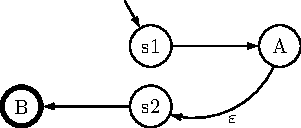
\includegraphics[width=\textwidth]{pics/mp/nfa-6.pdf}
                \center $M$
            \end{minipage}
        \end{center}
        thus 
        \[
            L(M) = L(M_1) \circ L(M_2)  = \set{wv \mid w \in L(M_1), v \in L(M_2)}
        \]
    \end{proof}
\end{example}


